\hypertarget{gtkapplication-and-gtkapplicationwindow}{%
\section{GtkApplication and
GtkApplicationWindow}\label{gtkapplication-and-gtkapplicationwindow}}

\hypertarget{gtkapplication}{%
\subsection{GtkApplication}\label{gtkapplication}}

\hypertarget{gtkapplication-and-g_application_run}{%
\subsubsection{GtkApplication and
g\_application\_run}\label{gtkapplication-and-g_application_run}}

Usually people write programming code to make an application. What are
applications? Applications are software that runs using libraries, which
includes the OS, frameworks and so on. In Gtk4 programming, the
GtkApplication is a program (or executable) that runs using Gtk
libraries.

The basic way to write a GtkApplication is as follows.

\begin{itemize}
\tightlist
\item
  Create a GtkApplication instance.
\item
  Run the application.
\end{itemize}

That's all. Very simple. The following is the C code representing the
scenario above.

\begin{lstlisting}[language=C, numbers=left]
#include <gtk/gtk.h>

int
main (int argc, char **argv) {
  GtkApplication *app;
  int stat;

  app = gtk_application_new ("com.github.ToshioCP.pr1", G_APPLICATION_FLAGS_NONE);
  stat =g_application_run (G_APPLICATION (app), argc, argv);
  g_object_unref (app);
  return stat;
}
\end{lstlisting}

The first line says that this program includes the header files of the
Gtk libraries. The function \passthrough{\lstinline!main!} above is a
startup function in C language. The variable
\passthrough{\lstinline!app!} is defined as a pointer to a
GtkApplication instance. The function
\passthrough{\lstinline!gtk\_application\_new!} creates a GtkApplication
instance and returns a pointer to the instance. The GtkApplication
instance is a C structure data in which the information about the
application is stored. The meaning of the arguments will be explained
later. The function \passthrough{\lstinline!g\_application\_run!} runs
an application that the instance defined. (We often say that the
function runs \passthrough{\lstinline!app!}. Actually,
\passthrough{\lstinline!app!} is not an application but a pointer to the
instance of the application. However, it is simple and short, and
probably no confusion occurs.)

To compile this, the following command needs to be run. The string
\passthrough{\lstinline!pr1.c!} is the filename of the C source code
above.

\begin{lstlisting}
$ gcc `pkg-config --cflags gtk4` pr1.c `pkg-config --libs gtk4`
\end{lstlisting}

The C compiler gcc generates an executable file,
\passthrough{\lstinline!a.out!}. Let's run it.

\begin{lstlisting}
$ ./a.out

(a.out:13533): GLib-GIO-WARNING **: 15:30:17.449: Your application does not implement
g_application_activate() and has no handlers connected to the "activate" signal.
It should do one of these.
$
\end{lstlisting}

Oh, it just produces an error message. This error message means that the
GtkApplication object ran, without a doubt. Now, let's think about what
this message means.

\hypertarget{signal}{%
\subsubsection{signal}\label{signal}}

The message tells us that:

\begin{enumerate}
\def\labelenumi{\arabic{enumi}.}
\tightlist
\item
  The application GtkApplication doesn't implement
  \passthrough{\lstinline!g\_application\_activate()!},
\item
  It has no handlers connected to the ``activate'' signal, and
\item
  You will need to solve at least one of these.
\end{enumerate}

These two causes of the error are related to signals. So, I will explain
that to you first.

A signal is emitted when something happens. For example, a window is
created, a window is destroyed and so on. The signal ``activate'' is
emitted when the application is activated, or started. If the signal is
connected to a function, which is called a signal handler or simply
handler, then the function is invoked when the signal emits.

The flow is like this:

\begin{enumerate}
\def\labelenumi{\arabic{enumi}.}
\tightlist
\item
  Something happens.
\item
  If it's related to a certain signal, then the signal is emitted.
\item
  If the signal as been connected to a handler, then the handler is
  invoked.
\end{enumerate}

Signals are defined in objects. For example, the ``activate'' signal
belongs to the GApplication object, which is a parent object of
GtkApplication object.

The GApplication object is a child object of the GObject object. GObject
is the top object in the hierarchy of all the objects.

\begin{lstlisting}
GObject -- GApplication -- GtkApplication
<---parent                      --->child
\end{lstlisting}

A child object inherits signals, functions, properties and so on from
its parent object. So, GtkApplication also has the ``activate'' signal.

Now we can solve the problem in \passthrough{\lstinline!pr1.c!}. We need
to connect the ``activate'' signal to a handler. We use a function
\passthrough{\lstinline!g\_signal\_connect!} which connects a signal to
a handler.

\begin{lstlisting}[language=C, numbers=left]
#include <gtk/gtk.h>

static void
app_activate (GApplication *app, gpointer *user_data) {
  g_print ("GtkApplication is activated.\n");
}

int
main (int argc, char **argv) {
  GtkApplication *app;
  int stat;

  app = gtk_application_new ("com.github.ToshioCP.pr2", G_APPLICATION_FLAGS_NONE);
  g_signal_connect (app, "activate", G_CALLBACK (app_activate), NULL);
  stat =g_application_run (G_APPLICATION (app), argc, argv);
  g_object_unref (app);
  return stat;
}
\end{lstlisting}

First, we define the handler \passthrough{\lstinline!app\_activate!}
which simply displays a message. In the function
\passthrough{\lstinline!main!}, we add
\passthrough{\lstinline!g\_signal\_connect!} before
\passthrough{\lstinline!g\_application\_run!}. The function
\passthrough{\lstinline!g\_signal\_connect!} has four arguments.

\begin{enumerate}
\def\labelenumi{\arabic{enumi}.}
\tightlist
\item
  An instance to which the signal belongs.
\item
  The name of the signal.
\item
  A handler function (also called callback), which needs to be casted by
  \passthrough{\lstinline!G\_CALLBACK!}.
\item
  Data to pass to the handler. If no data is necessary, NULL should be
  given.
\end{enumerate}

You can find the description of each signal in the API reference manual.
For example, ``activate'' signal is in GApplication section in
\href{https://docs.gtk.org/gio/signal.Application.activate.html}{GIO API
Reference}. The handler function is described in it.

In addition, \passthrough{\lstinline!g\_signal\_connect!} is described
in \href{https://docs.gtk.org/gobject/func.signal_connect.html}{GObject
API Reference}. API reference manual is very important. You should see
and understand it to write Gtk applications. They are located in
\href{https://docs.gtk.org/}{`GTK Documentation'}.

Let's compile the source file above (\passthrough{\lstinline!pr2.c!})
and run it.

\begin{lstlisting}
$ gcc `pkg-config --cflags gtk4` pr2.c `pkg-config --libs gtk4`
$ ./a.out
GtkApplication is activated.
$
\end{lstlisting}

OK, well done. However, you may have noticed that it's painful to type
such a long line to compile. It is a good idea to use shell script to
solve this problem. Make a text file which contains the following line.

\begin{lstlisting}
gcc `pkg-config --cflags gtk4` $1.c `pkg-config --libs gtk4`
\end{lstlisting}

Then, save it under the directory \$HOME/bin, which is usually
/home/(username)/bin. (If your user name is James, then the directory is
/home/james/bin). And turn on the execute bit of the file. If the
filename is \passthrough{\lstinline!comp!}, do like this:

\begin{lstlisting}
$ chmod 755 $HOME/bin/comp
$ ls -log $HOME/bin
    ...  ...  ...
-rwxr-xr-x 1   62 May 23 08:21 comp
    ...  ...  ...
\end{lstlisting}

If this is the first time that you make a \$HOME/bin directory and save
a file in it, then you need to logout and login again.

\begin{lstlisting}
$ comp pr2
$ ./a.out
GtkApplication is activated.
$
\end{lstlisting}

\hypertarget{gtkwindow-and-gtkapplicationwindow}{%
\subsection{GtkWindow and
GtkApplicationWindow}\label{gtkwindow-and-gtkapplicationwindow}}

\hypertarget{gtkwindow}{%
\subsubsection{GtkWindow}\label{gtkwindow}}

A message ``GtkApplication is activated.'' was printed out in the
previous subsection. It was good in terms of a test of GtkApplication.
However, it is insufficient because Gtk is a framework for graphical
user interface (GUI). Now we go ahead with adding a window into this
program. What we need to do is:

\begin{enumerate}
\def\labelenumi{\arabic{enumi}.}
\tightlist
\item
  Create a GtkWindow.
\item
  Connect it to GtkApplication.
\item
  Show the window.
\end{enumerate}

Now rewrite the function \passthrough{\lstinline!app\_activate!}.

\hypertarget{create-a-gtkwindow}{%
\paragraph{Create a GtkWindow}\label{create-a-gtkwindow}}

\begin{lstlisting}[language=C, numbers=left]
static void
app_activate (GApplication *app, gpointer user_data) {
  GtkWidget *win;

  win = gtk_window_new ();
  gtk_window_set_application (GTK_WINDOW (win), GTK_APPLICATION (app));
  gtk_widget_show (win);
}
\end{lstlisting}

Widget is an abstract concept that includes all the GUI interfaces such
as windows, dialogs, buttons, multi-line text, containers and so on. And
GtkWidget is a base object from which all the GUI objects derive.

\begin{lstlisting}
parent <-----> child
GtkWidget -- GtkWindow
\end{lstlisting}

GtkWindow includes GtkWidget at the top of its object.

\begin{figure}
\centering
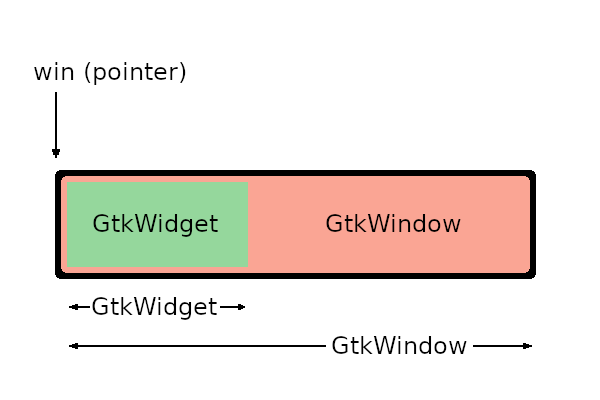
\includegraphics[width=9cm,height=6cm]{../image/window_widget.png}
\caption{GtkWindow and GtkWidget}
\end{figure}

The function \passthrough{\lstinline!gtk\_window\_new!} is defined as
follows.

\begin{lstlisting}[language=C]
GtkWidget *
gtk_window_new (void);
\end{lstlisting}

By this definition, it returns a pointer to GtkWidget, not GtkWindow. It
actually creates a new GtkWindow instance (not GtkWidget) but returns a
pointer to GtkWidget. However,the pointer points the GtkWidget and at
the same time it also points GtkWindow that contains GtkWidget in it.

If you want to use \passthrough{\lstinline!win!} as a pointer to the
GtkWindow, you need to cast it.

\begin{lstlisting}[language=C]
(GtkWindow *) win
\end{lstlisting}

Or you can use \passthrough{\lstinline!GTK\_WINDOW!} macro that performs
a similar function.

\begin{lstlisting}[language=C]
GTK_WINDOW (win)
\end{lstlisting}

This is a recommended way.

\hypertarget{connect-it-to-gtkapplication.}{%
\paragraph{Connect it to
GtkApplication.}\label{connect-it-to-gtkapplication.}}

The function \passthrough{\lstinline!gtk\_window\_set\_application!} is
used to connect GtkWindow to GtkApplication.

\begin{lstlisting}[language=C]
gtk_window_set_application (GTK_WINDOW (win), GTK_APPLICATION (app));
\end{lstlisting}

You need to cast \passthrough{\lstinline!win!} to GtkWindow and
\passthrough{\lstinline!app!} to GtkApplication.
\passthrough{\lstinline!GTK\_WINDOW!} and
\passthrough{\lstinline!GTK\_APPLICATION!} macro is appropriate for
that.

GtkApplication continues to run until the related window is destroyed.
If you didn't connect GtkWindow and GtkApplication, GtkApplication
destroys itself immediately. Because no window is connected to
GtkApplication, GtkApplication doesn't need to wait anything. As it
destroys itself, the GtkWindow is also destroyed.

\hypertarget{show-the-window.}{%
\paragraph{Show the window.}\label{show-the-window.}}

The function \passthrough{\lstinline!gtk\_widget\_show!} is used to show
the window.

Gtk4 changes the default widget visibility to on, so every widget
doesn't need this function to show itself. But, there's an exception.
Top window (this term will be explained later) isn't visible when it is
created. So you need to use the function above to show the window.

Save the program as \passthrough{\lstinline!pr3.c!} and compile and run
it.

\begin{lstlisting}
$ comp pr3
$ ./a.out
\end{lstlisting}

A small window appears.

\begin{figure}
\centering

\includegraphics[width=3.3cm,height=3.825cm]{../image/screenshot_pr3.png}
\caption{Screenshot of the window}
\end{figure}

Click on the close button then the window disappears and the program
finishes.

\hypertarget{gtkapplicationwindow}{%
\subsubsection{GtkApplicationWindow}\label{gtkapplicationwindow}}

GtkApplicationWindow is a child object of GtkWindow. It has some extra
functionality for better integration with GtkApplication. It is
recommended to use it instead of GtkWindow when you use GtkApplication.

Now rewrite the program and use GtkApplicationWindow.

\begin{lstlisting}[language=C, numbers=left]
static void
app_activate (GApplication *app, gpointer user_data) {
  GtkWidget *win;

  win = gtk_application_window_new (GTK_APPLICATION (app));
  gtk_window_set_title (GTK_WINDOW (win), "pr4");
  gtk_window_set_default_size (GTK_WINDOW (win), 400, 300);
  gtk_widget_show (win);
}
\end{lstlisting}

When you create GtkApplicationWindow, you need to give GtkApplication
instance as an argument. Then it automatically connect these two
instances. So you don't need to call
\passthrough{\lstinline!gtk\_window\_set\_application!} any more.

The program sets the title and the default size of the window. Compile
it and run \passthrough{\lstinline!a.out!}, then you will see a bigger
window with its title ``pr4''.

\begin{figure}
\centering
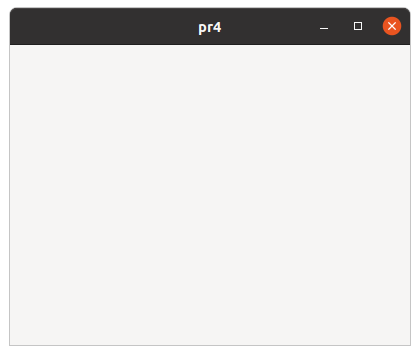
\includegraphics[width=6.3cm,height=5.325cm]{../image/screenshot_pr4.png}
\caption{Screenshot of the window}
\end{figure}
